\documentclass[UTF8]{ctexart}
\usepackage{ctex}
\usepackage{amsmath}
\usepackage{amsthm}
\usepackage{geometry}
\geometry{left=2.5cm,right=2.5cm,top=2.5cm,bottom=2.5cm}
\usepackage{amssymb}
\usepackage{indentfirst}
\usepackage{graphicx}
\usepackage{subfigure}
\usepackage{listings}
\usepackage{xcolor}
\usepackage{float}
\usepackage{algorithm}  
\usepackage{algorithmicx}  
\usepackage{longtable}
\usepackage{fancyhdr}
\usepackage{appendix}
\usepackage{enumitem}
\usepackage{abstract}
\usepackage{multirow}
\pagestyle{fancy}
\lfoot{}%这条语句可以让页码出现在下方
\theoremstyle{plain}
\newtheorem{thm}{Theorem}[section]
\newtheorem{lem}[thm]{Lemma}
\newtheorem{prop}[thm]{Proposition}
\newtheorem{cor}[thm]{Corollary}

\theoremstyle{definition}
\newtheorem{defn}{Definition}[section]

\theoremstyle{remark}
\newtheorem*{rem}{Remark}
\newtheorem{eg}{Example}[section]
\title{Design document}
\author{Shuang Hu}
\begin{document}
\maketitle
Here are the descriptions of my program.
\section*{Class Mesh}
The mesh class is designed to store the mesh used in the 1D BVP. It contains following protected elements:
\begin{itemize}
\item n: means the number of intervals.
\item nodes: means the approximated value of $u(x_{i})$ on plot $x_{i}$.
\item size: means the size of vector 'nodes'.
\end{itemize}

The member function of such class:
\begin{itemize}
\item Mesh(int sz): Construct a mesh object with size sz.
\item void setsize(int sz): Set the size of the object.
\item void setzero(): Set the elements of vector nodes to zero.
\item int getsize(): Get the size of mesh.
\item valarray<double> getinfo(): Get the vector nodes.
\item void setinfo(valarray<double> vec): Set the value of vector nodes same as vec.
\item virtual void tocoarse()=0: Achieve operator $I_{h}^{2h}$ with different types.
\item virtual void torefine()=0: Achieve operator $I_{2h}^{h}$ with different types.
\item void printMesh(): Print the information of nodes.
\end{itemize}

By the different choice of refine/coarse operator, there are 4 derived classes of class Mesh. They are defined as \textbf{Meshtype1}, \textbf{Meshtype2}, \textbf{Meshtype3} and \textbf{Meshtype4}.
\section*{Class VCycle}
The VCycle class is designed to achieve V-Cycle algorithm, then solve the BVP by multigrid method. It contains following protected elements:
\begin{itemize}
\item Mesh M: A mesh to store the result.
\item int mu1,mu2: Smooth times of Weighted-Jacobi method.
\item double LeftBC,RightBC: Boundary condition.
\item valarray<double> Righthand: the righthand vector $f$ in linear system.
\item double maxerror: The maximum agreed relative error.
\end{itemize}

The member function:
\begin{itemize}
\item VCycle(int sz,int mu1,int mu2): Constructor function. Set the information of mesh M, smooth times mu1 and mu2.
\item void seterr(double e): Set the maximal error.
\item void setmesh(Mesh\& m1): Set the value of mesh.
\item Mesh\& getmesh(): Get the information of mesh.
\item Mesh\& WeightedJacob(int mu,Mesh\& M,valarray<double>\& Righthand): Achieve the Weighted-Jacobian iteration algorithm.
\item void setBC(double L,double R): Set the boundary condition of the BVP.
\item valarray<double> generateRH(Mesh\& M): Get the right-hand vector $f$.
\item valarray<double> Residure(valarray<double>\& f1,valarray<double>\& v1): Get the residure vector $e$.
\item Mesh\& cycle(Mesh\& M,valarray<double>\& f): Achieve VCycle algorithm.
\item void getresult(): Output the final Matlab file.
\item double generateerror(): Get the relative error.
\item bool quit(): Judge quit the VCycle loop or not.
\end{itemize}
\section*{Class FMG}

The FMG class is derived from VCycle. It is made to achieve full multigrid cycle.

Member:
\begin{itemize}
\item Mesh\& FMGcycle(valarray<double>\& f,int vcycletimes): Achieve FMG algorithm.
\end{itemize}
\section*{UML diagram}
\begin{figure}[H]
\centering
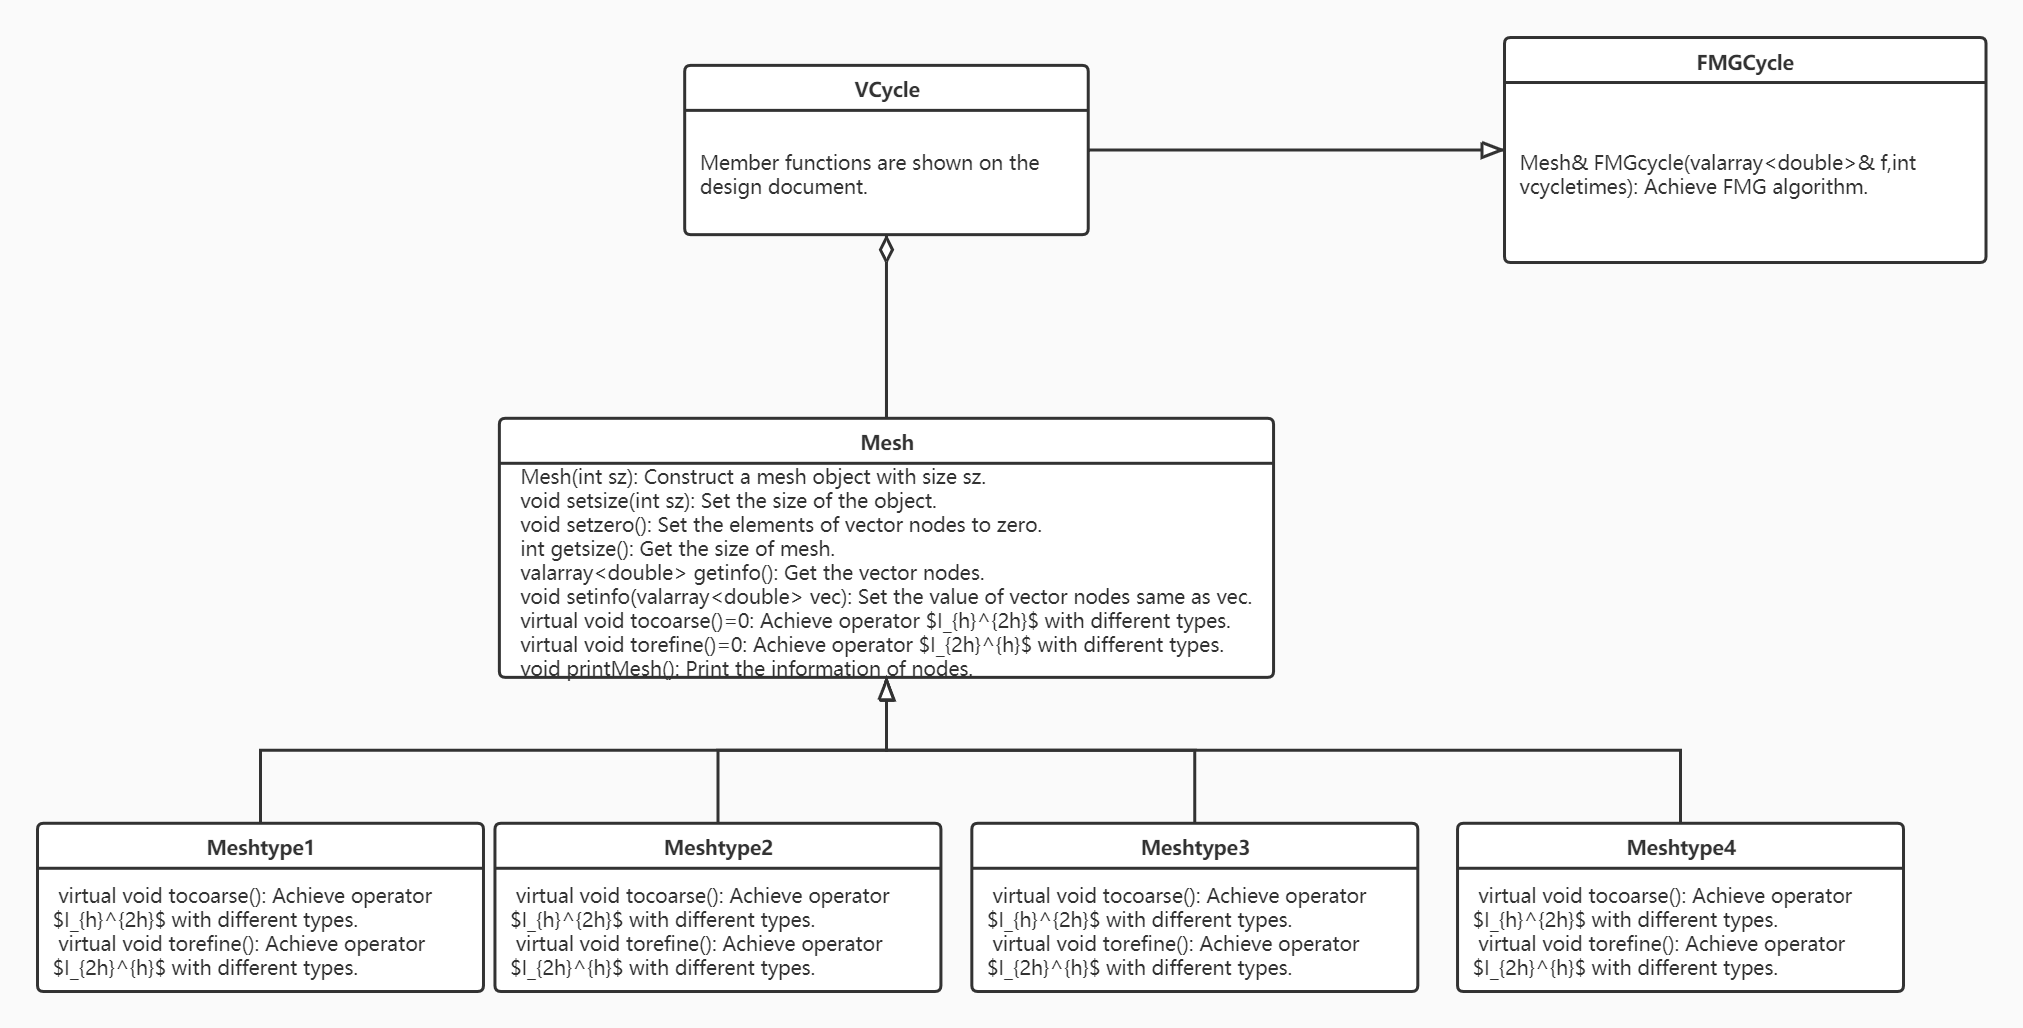
\includegraphics[height=0.4\textheight,width=0.8\linewidth]{UML}
\caption{UML diagram.}
\end{figure}

\textbf{Remark:} 4 different type of mesh haven't done yet.
\end{document}